% !TEX root = main.tex
\section{Judge Certification: Additional Plots}\label{app:judge-cert}
We report raw scatterplots used during certification of the LLM judge.
These plots visualize the judge’s response to controlled perturbations: (P1) identity/reflexivity, (P2) cumulative bug injection, and (P3) removal of theorem statements and unit tests.
Figures A.1–A.3 show that scores drop as artifacts worsen; the bug plot is noisier with an early prompt, which motivated the simplified rubric used in the main experiments.
P4 (prompt stability/invariance) is reported in the main text with dedicated aggregate plots.

\textit{Protocol variants.} The scatterplots below are “sanity-check” runs with the simplest prompts to stress visible monotonic behavior.
In the bug study (Fig.~\ref{fig:app-bugs}) the earlier, theorem-equivalence prompt produced a noisier trend; this prompted a simplified, rubric-first prompt that we use for all reported results in the main paper, yielding the stronger correlations cited in Fig.~\ref{fig:judge_sanity_checks}.
For missing-specs (Fig.~\ref{fig:app-missing-specs}), both Claude 3.5 and 3.7 show clear negative trends; minor non-monotonicity in 3.7 disappears with the finalized rubric.

We note that, for the experiment shown in Figure \ref{fig:app-missing-specs}, a more complex judge (Claude 3.7) does not satisfy the property that the LLM Judge Score should monotonically decrease with the number of missing specs.
Indeed, the Judge File Equivalence score was not monotonic, even for Claude 3.5, leading us to simplify the rubric used in our main paper.

\begin{figure}[t]
  \centering
  \begin{subfigure}[t]{0.48\textwidth}
    \centering
    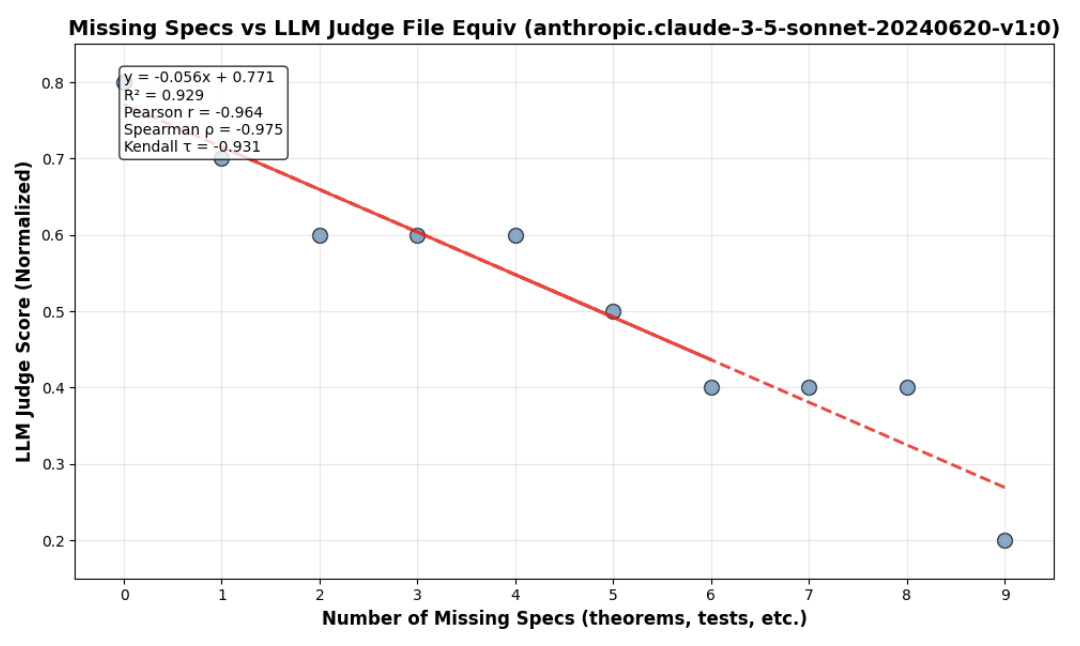
\includegraphics[width=\linewidth]{figures/3.5_specs_missing.png}
    \caption{Claude 3.5 Sonnet v1: strong monotonic decrease (\(y=-0.056x+0.771\), \(R^2=0.929\), Pearson \(r=-0.964\), Spearman \(\rho=-0.975\)).}
  \end{subfigure}\hfill
  \begin{subfigure}[t]{0.48\textwidth}
    \centering
    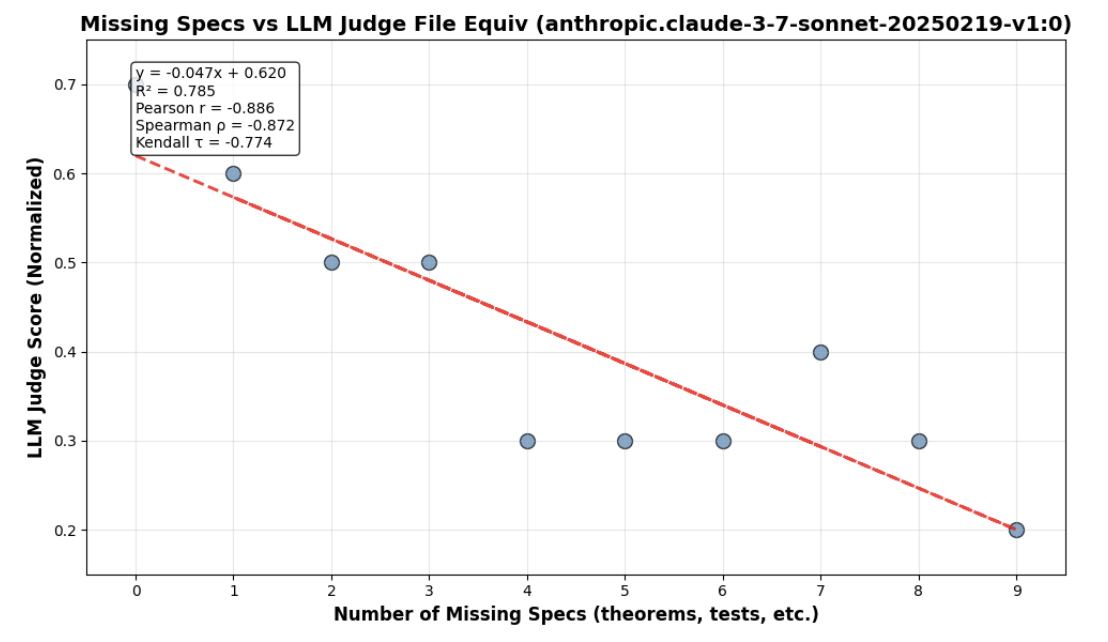
\includegraphics[width=\linewidth]{figures/3.7_specs_missing.png}
    \caption{Claude 3.7 Sonnet v1: clear negative trend with minor non-monotonicity (\(y=-0.047x+0.620\), \(R^2=0.785\), Pearson \(r=-0.886\), Spearman \(\rho=-0.872\)).}
  \end{subfigure}
  \caption{\textbf{(P3) Monotonicity w.r.t.\ missing specifications.} Candidate scores decrease as more theorems/tests are withheld.
  We retain both model variants to show robustness of the trend; 3.7’s small non-monotonicity motivated the simplified rubric used in the main results.}
  \label{fig:app-missing-specs}
\end{figure}

\begin{figure}[t]
  \centering
  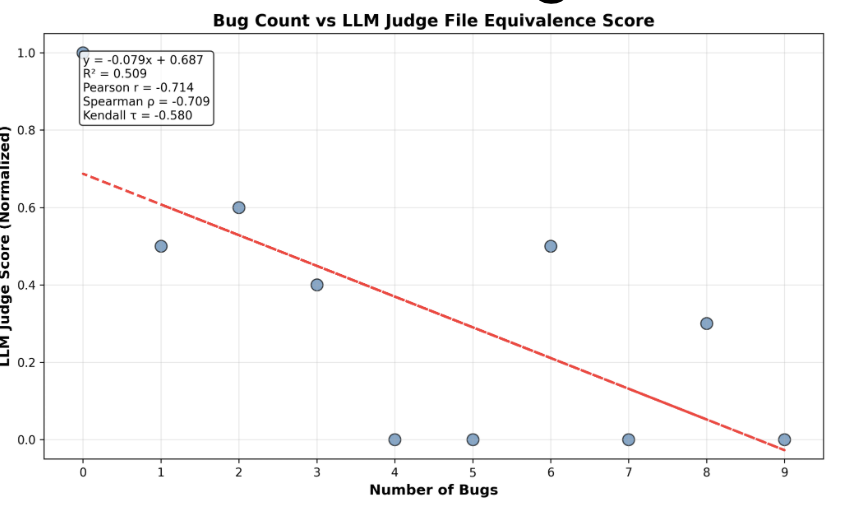
\includegraphics[width=0.85\linewidth]{figures/3.5_bugs.png}
  \caption{\textbf{(P2) Non-Monotonicity w.r.t.\ cumulative bugs (Claude 3.5 Sonnet).} Scores drop as more semantic bugs are injected (Pearson \(r=-0.714\), Spearman \(\rho=-0.709\), \(R^2=0.509\)); the higher noise with the initial “theorem-equivalence” prompt led us to simplify the rubric used for the final judge in the main paper.}
  \label{fig:app-bugs}
\end{figure}

\begin{figure}[t]
  \centering
  \begin{subfigure}[t]{0.49\textwidth}
    \centering
    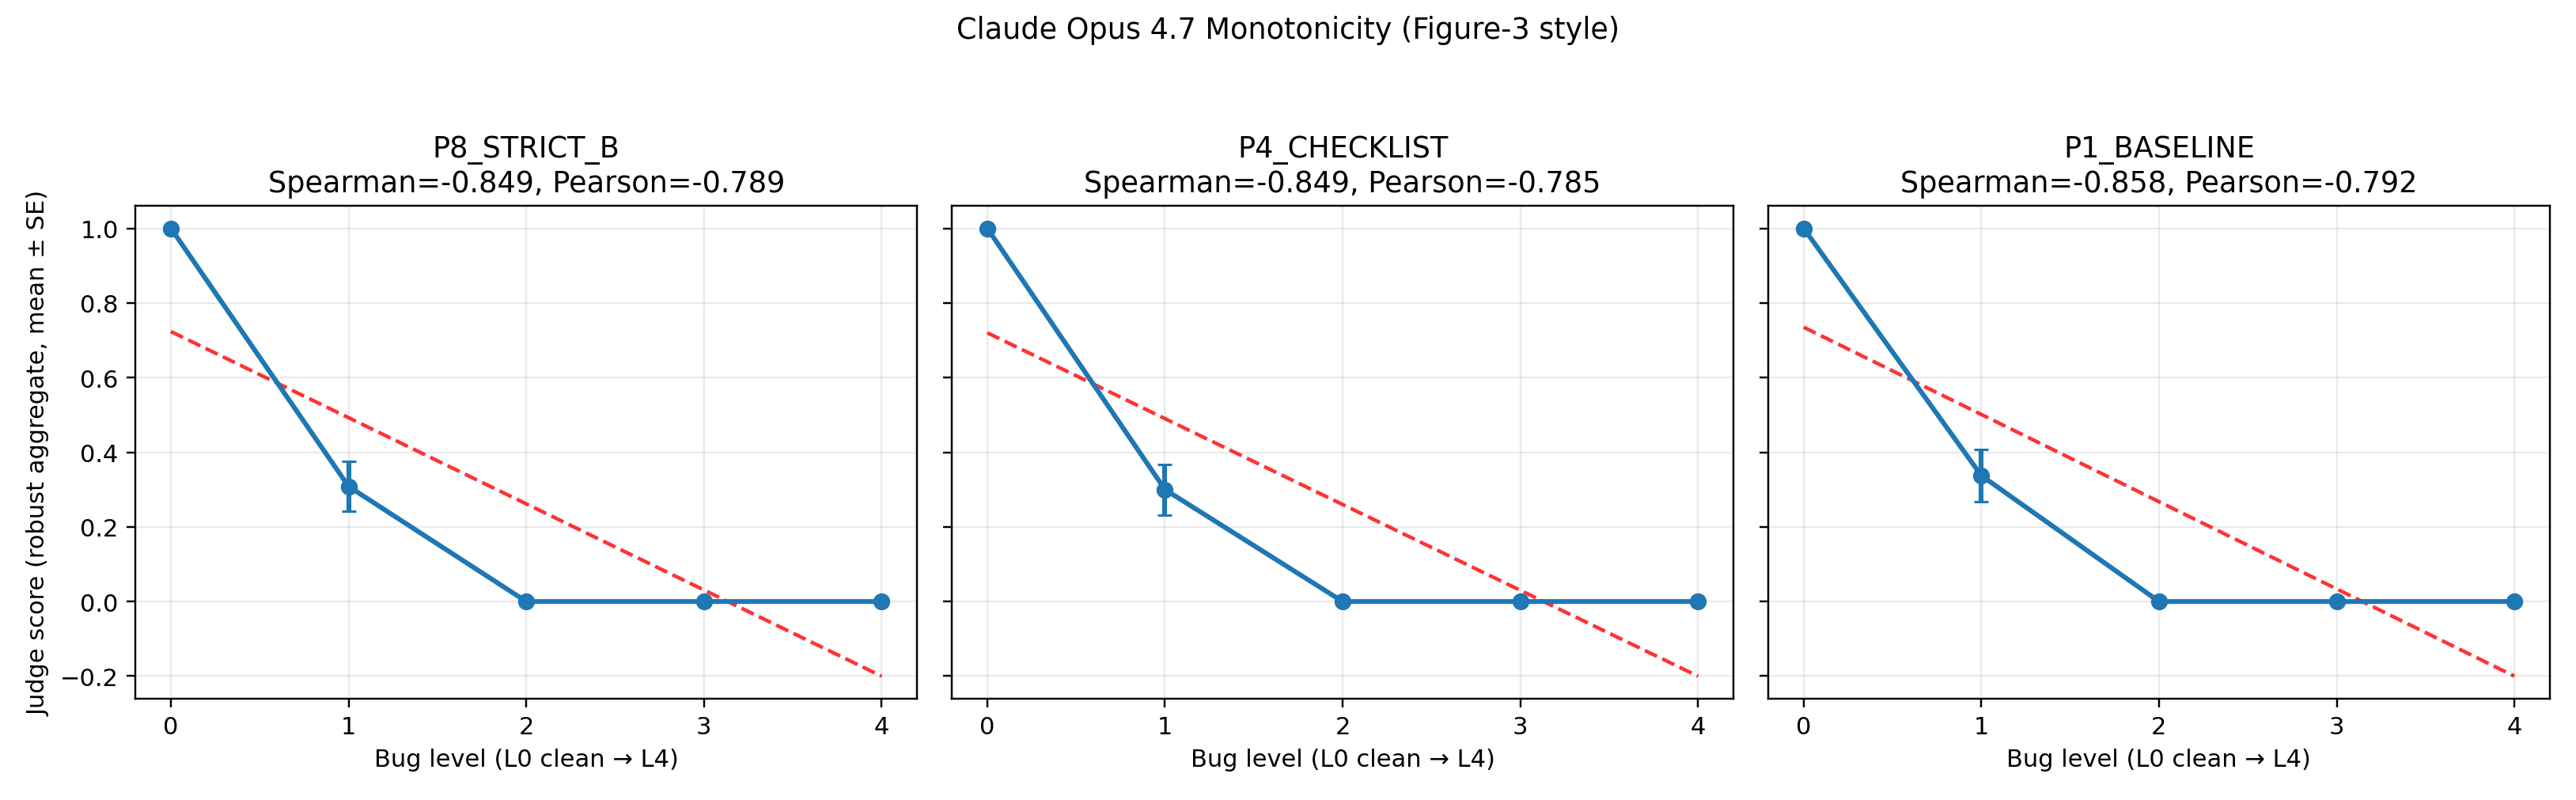
\includegraphics[width=\linewidth]{figures/fig3_style_claude_opus_monotonicity.png}
    \caption{Claude Opus 4.7 Figure-3-style monotonicity (mean \(\pm\) SE).}
  \end{subfigure}\hfill
  \begin{subfigure}[t]{0.49\textwidth}
    \centering
    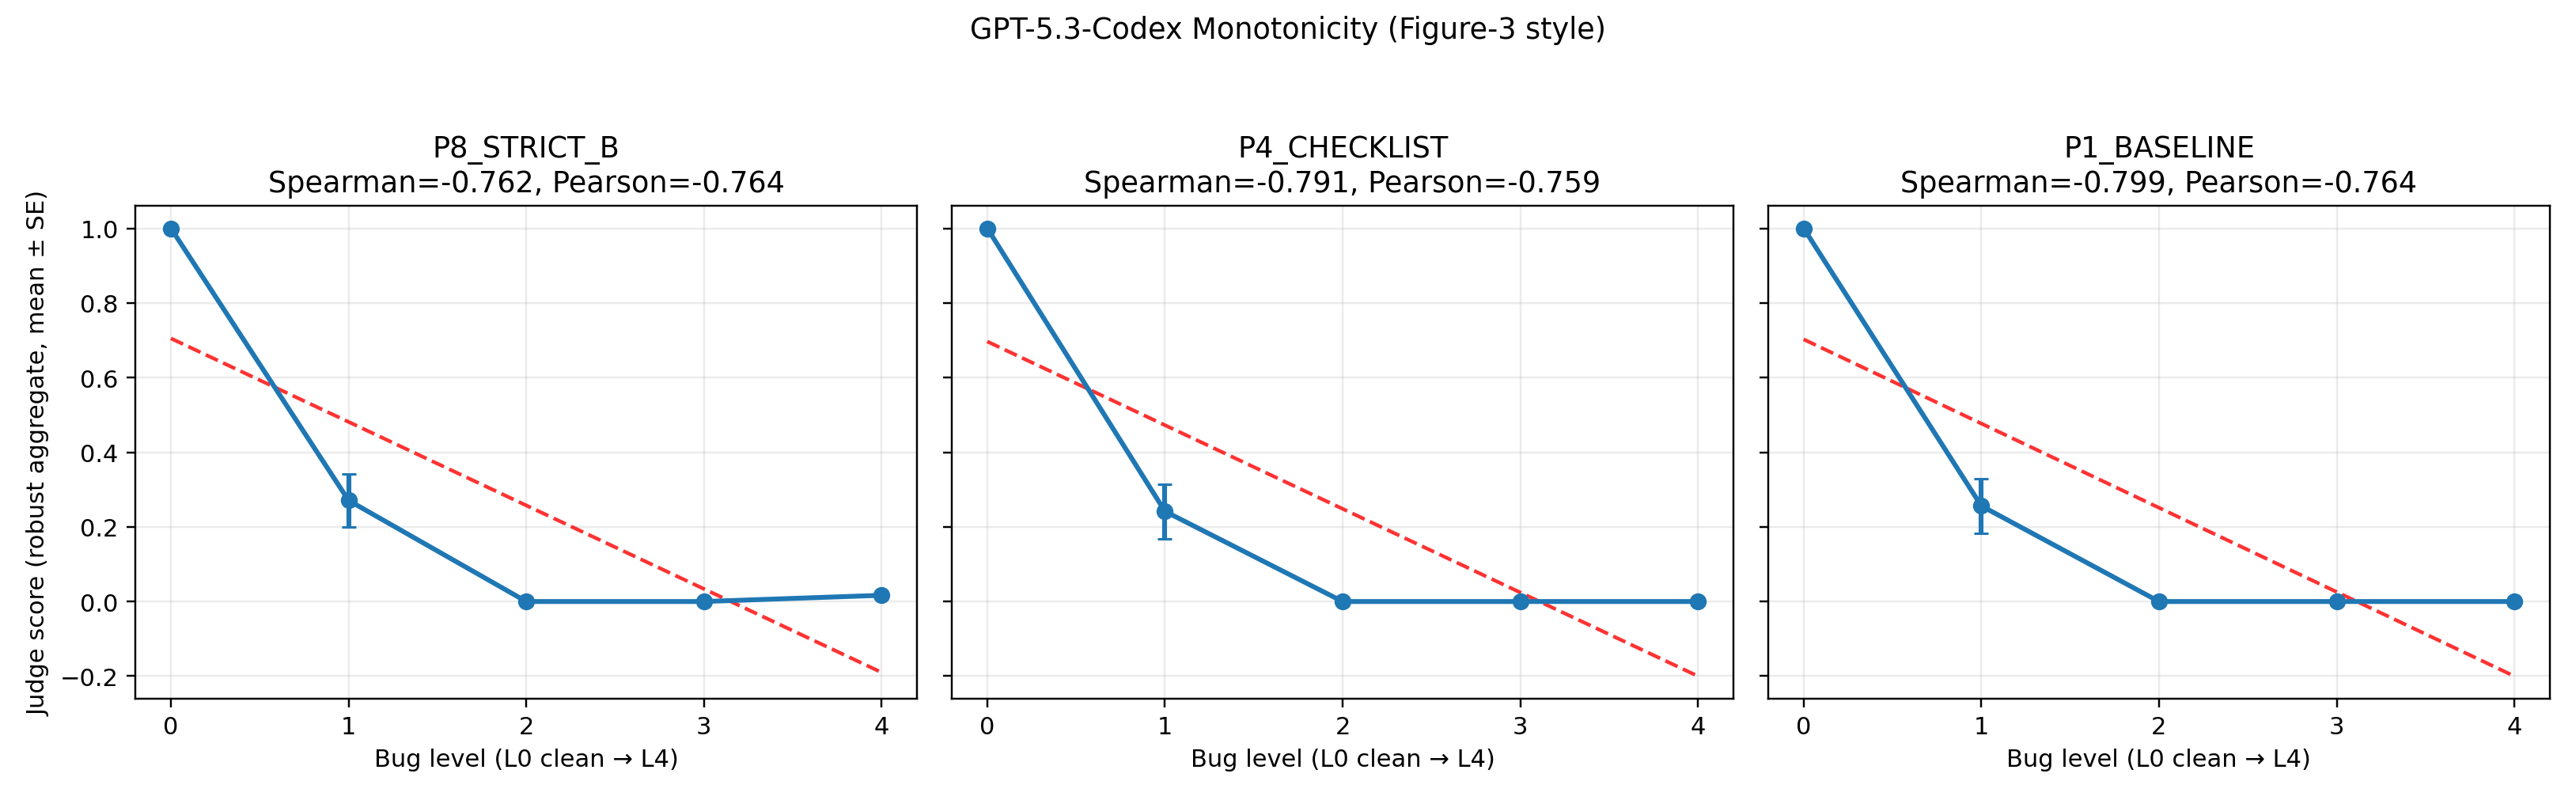
\includegraphics[width=\linewidth]{figures/fig3_style_gpt53_codex_monotonicity.png}
    \caption{GPT-5.3-Codex Figure-3-style monotonicity (mean \(\pm\) SE).}
  \end{subfigure}
  \caption{\textbf{Model-matched Figure-3-style monotonicity diagnostics.} Both judge families show strong monotone score degradation as bug intensity increases, under the same low-variance plotting protocol.}
  \label{fig:fig3_style_opus_codex}
\end{figure}

\begin{figure}[t]
  \centering
  \begin{subfigure}[t]{0.49\textwidth}
    \centering
    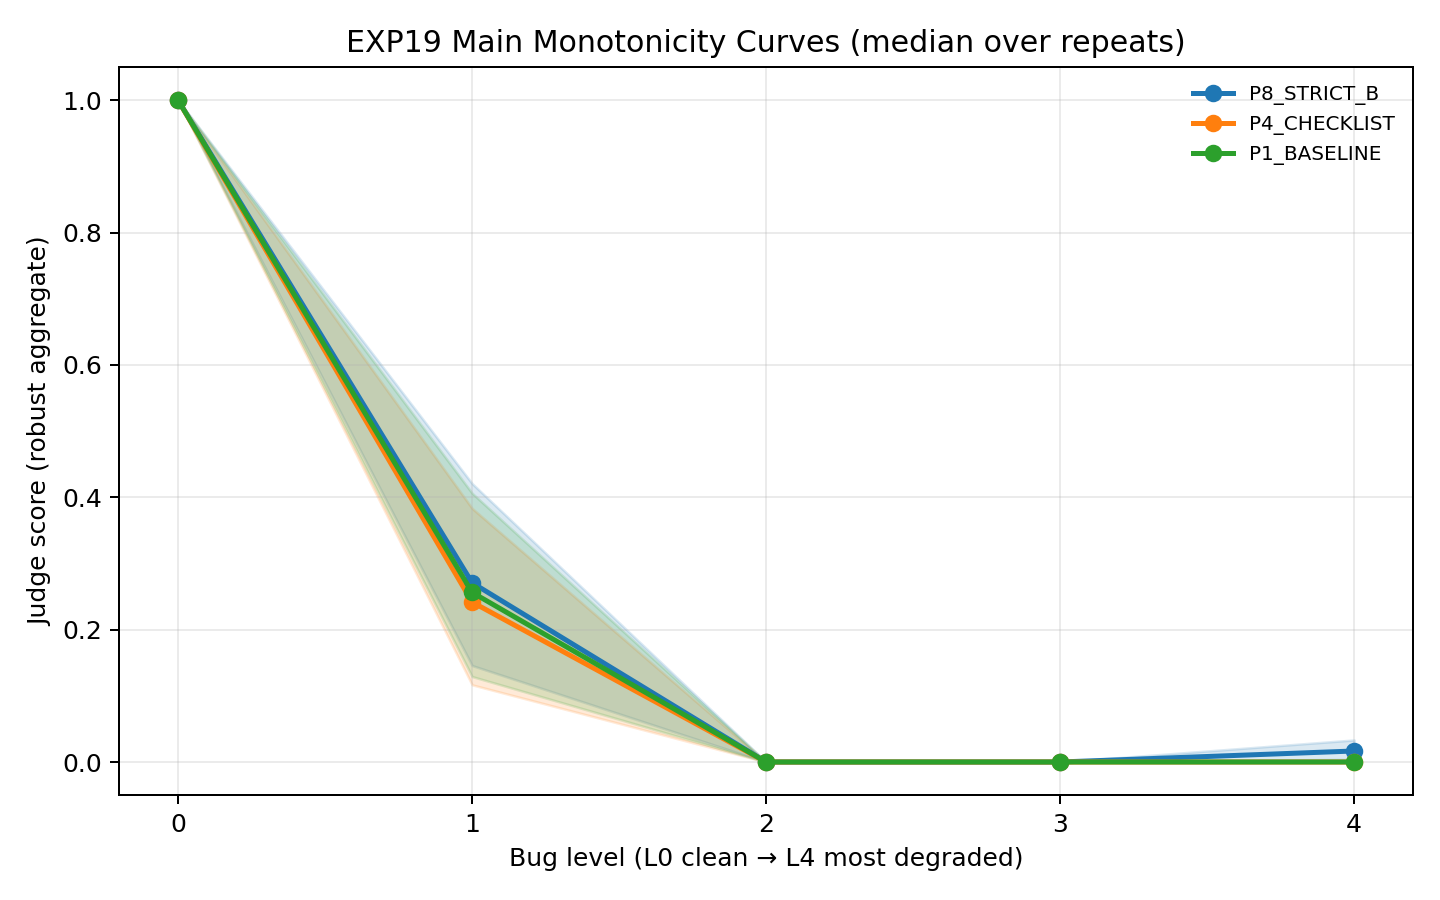
\includegraphics[width=\linewidth]{figures/fig_main_monotonicity_lowvar_codex.png}
    \caption{Codex low-variance monotonicity curves.}
  \end{subfigure}\hfill
  \begin{subfigure}[t]{0.49\textwidth}
    \centering
    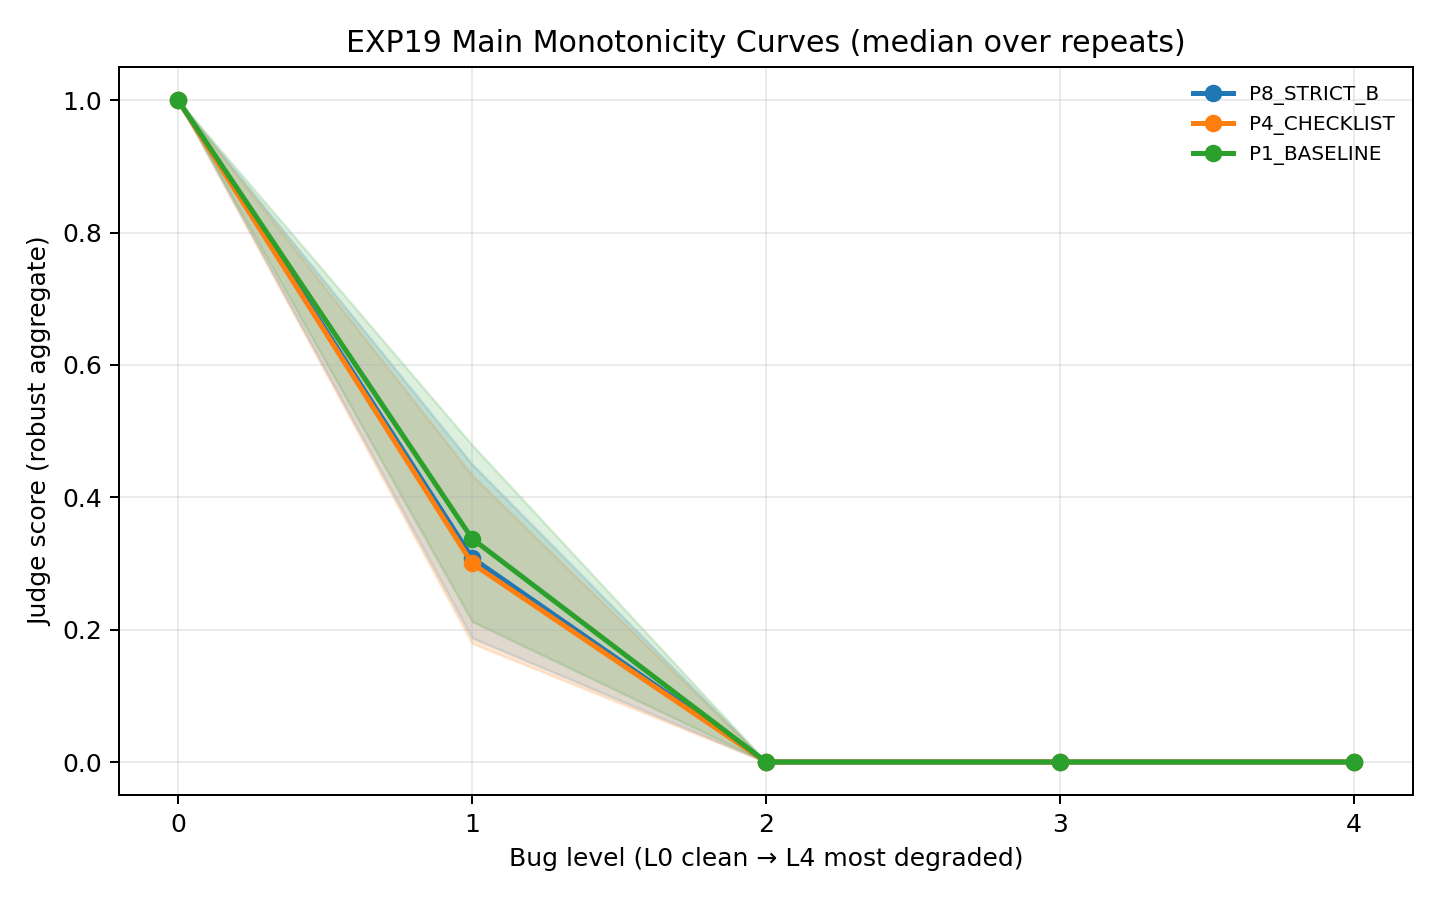
\includegraphics[width=\linewidth]{figures/fig_main_monotonicity_lowvar_opus47.png}
    \caption{Opus 4.7 low-variance monotonicity curves.}
  \end{subfigure}
  \caption{\textbf{Low-variance monotonicity trends across model families.} Both judge families show strong non-increasing behavior as bug intensity increases, under robust repeat aggregation.}
  \label{fig:lowvar_mono_codex_opus}
\end{figure}

